\begin{frame}
\frametitle{TSR-TVD: Temporal Super-Resolution for Time-Varying Data Analysis and
    Visualization}
    \begin{itemize}
        \item HPC has issues with storing time-steps.
        \item Some researchers LERP between time-steps to find intermediate
        data.
        \item TSR-TVD is a machine learning implementation to synthesize
        timesteps.
        \item Researchers are modifying existing ML techniques to solve problems
        in HPC.
        \item https://ieeexplore.ieee.org/document/8802285
    \end{itemize}
\end{frame}

\begin{frame}
\frametitle{TSR-TVD: Temporal Super-Resolution for Time-Varying Data Analysis and
    Visualization}
    \center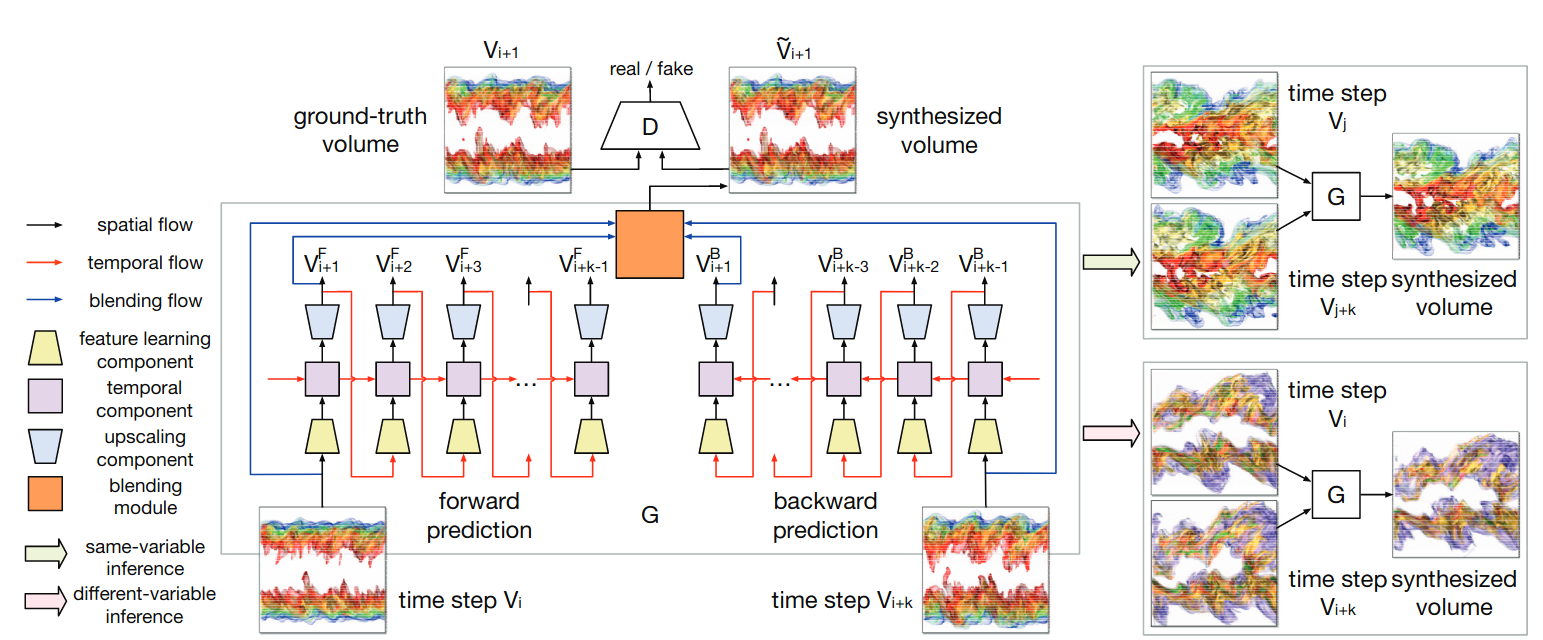
\includegraphics[width=0.9\paperwidth]{TSR.png}
\end{frame}

\begin{frame}
\frametitle{TSR-TVD: Temporal Super-Resolution for Time-Varying Data Analysis and
    Visualization}
    \begin{itemize}
        \item Uses RNN to create forward and backward predictions
        \item Conv3D GAN adversarially trains network.
        \item TSR-TVD uses structure similar to TecoGAN
    \end{itemize}
\end{frame}

\begin{frame}
\frametitle{TSR-TVD: Temporal Super-Resolution for Time-Varying Data Analysis and
    Visualization}
    \center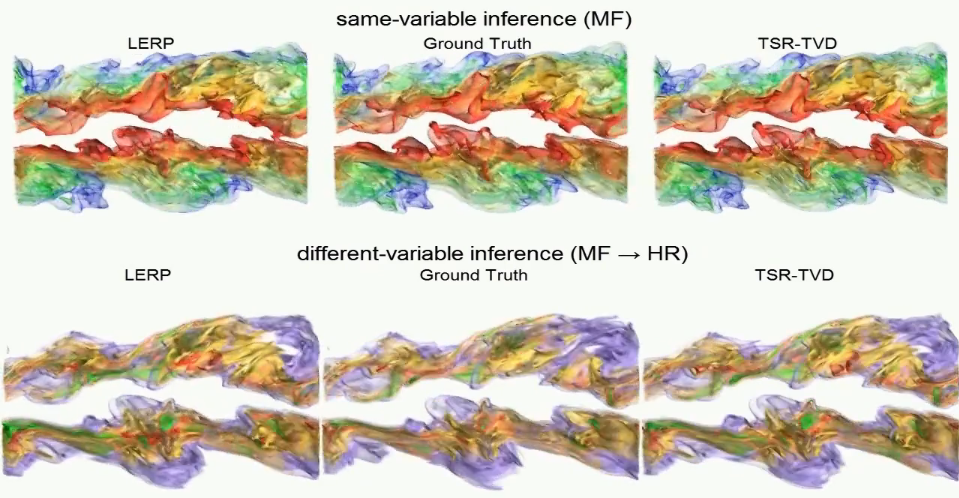
\includegraphics[width=0.8\paperwidth]{TSR_Link.png}
    \\
    \href{https://vimeo.com/359998660}{Short Video}\\ 
    https://vimeo.com/359998660
\end{frame}

\begin{frame}
\frametitle{TSR-TVD: Temporal Super-Resolution for Time-Varying Data Analysis and
    Visualization}
    \center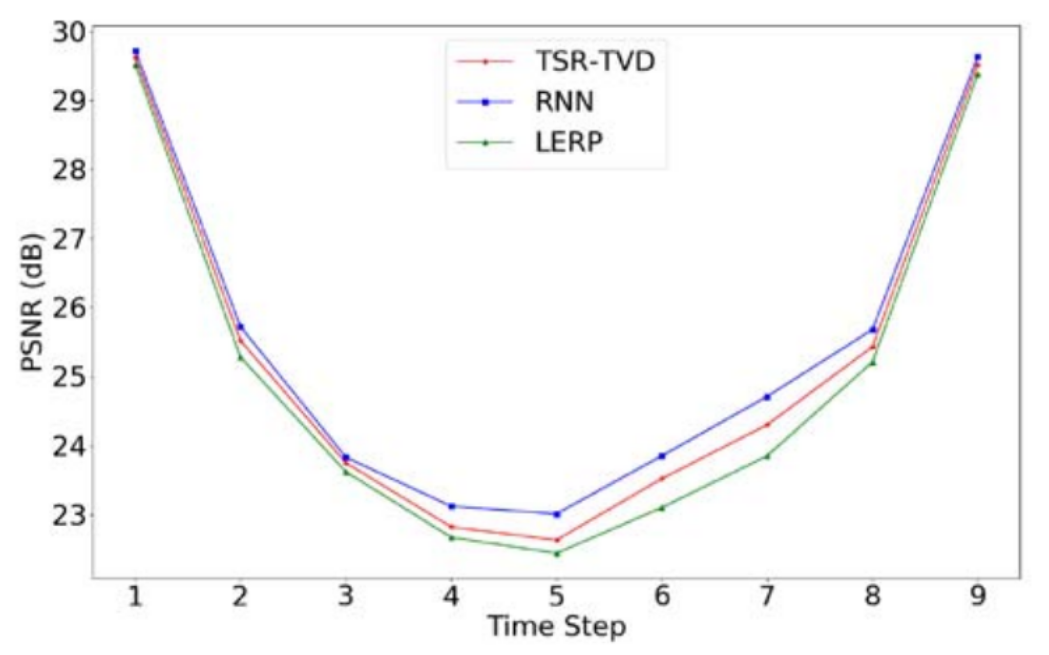
\includegraphics[width=0.8\paperwidth]{PSNR.png}
\end{frame}

